

\begin{frame}
\frametitle{Calibration : Goals}
The goal of the calibration effort was to improve near field, short time scale 
results of the analytic model using the numeric model.

The EBS responds to changes in the waste package decay heat more rapidly than 
the field in the surrounding host rock. This behavior is not taken into account
in the analytic model, but is explicitly accounted for in the numeric model. The following
simple empirical expression is plausibly added to the analytic model to more accurately
estimate temperatures at locations within storage drifts. 
\end{frame}

\begin{frame}

\frametitle{Calibration : Resistance Factor}

\footnotesize{
The difference in temperature due to the instantaneous transient response in the  
tunnel is here modeled as $\Delta T$, 

\begin{align}
  \Delta T(t) &= T_{numeric}(r_{t}) - T_{analytic}(\frac{D_d}{2})\\ 
  \Delta T(t) &= C q_L(t) 
  \frac{1}{K_{th}}\frac{1}{D_d}\\
  \intertext{where}
  D_{d} &= \mbox{Distance between drifts} [m]\nonumber\\
  r_{t} &= \mbox{Tunnel wall radius, calculation radius} [m]\nonumber
  \intertext{and}
  C &= \mbox{A coefficient derived from fitting}[m].\nonumber
  \label{deltat}
\end{align}

This allows the capacitive behavior of the model to remain entirely in the 
analytic model, and embeds the resistive behavior in a purely algebraic 
calibration. The calibration is valid for all repository configurations which 
share a tunnel diameter, tunnel spacing, and host rock material.
}
\end{frame}

\begin{frame}
  \frametitle{Calibration : Multiple Tunnel Results}
For a clay repository ($K_{th} = 2.5 [W\cdot m^{-1}\cdot K^{-1}$, $\alpha = 
1.13\times10^{-6}[m^2\cdot s^{-1}$), with a tunnel diameter of $0.7m$, the 
calibration was completed using a fit between a 101 drift analytic scenario 
and the numeric model with an infinite number of drifts. $D_{d}$, the drift 
spacing, was $30m$ in each case.

A fitting coefficient of $C=0.0265m$ improves agreement for the clay 
case with a $0.7m$ tunnel diameter and multiple drifts. The success of the fit 
decreases for longer cooling times.
\end{frame}

\begin{frame}[ctb!]
  \frametitle{100 Tunnel 10 year}
  \begin{figure}[h]
    \begin{center}
      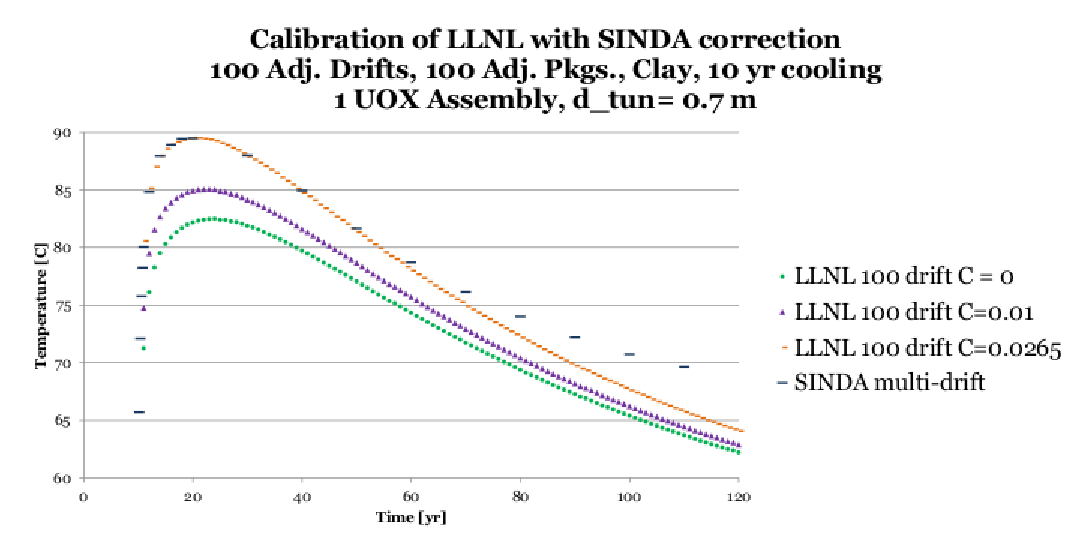
\includegraphics[width=.8\textwidth]{100drift10yr.eps}
      \caption{A multiple drift scenario approximated the inifinite repository 
      scenario run with the SINDA technique.}
    \end{center}
    \label{fig:100drift10yr}
  \end{figure}
\end{frame}

\begin{frame}[ctb!]
  \frametitle{100 Tunnel 25 year}
  \begin{figure}[h]
    \begin{center}
      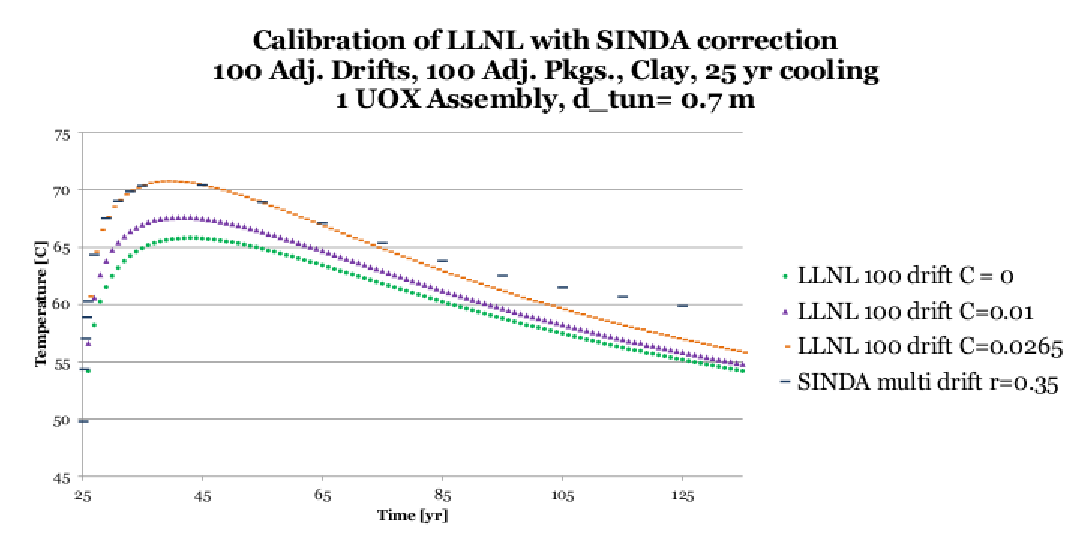
\includegraphics[width=.8\textwidth]{100drift25yr.eps}
      \caption{A multiple drift scenario approximated the inifinite repository 
      scenario run with the SINDA technique.}
    \end{center}
    \label{fig:100drift25yr}
  \end{figure}
  
\end{frame}
\begin{frame}[ctb!]

  \frametitle{100 Tunnel 50 year}
  \begin{figure}[h]
    \begin{center}
      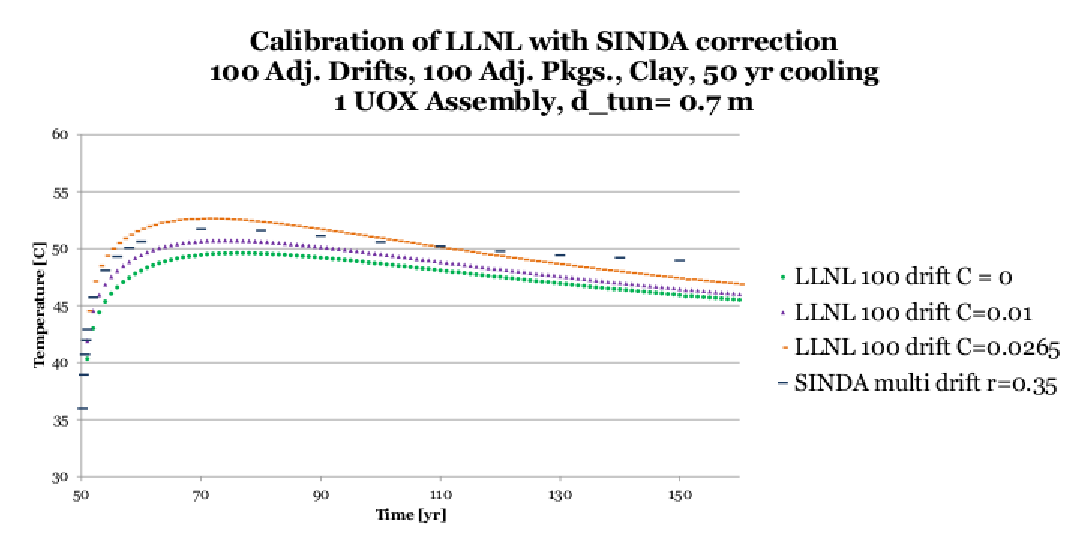
\includegraphics[width=.8\textwidth]{100drift50yr.eps}
      \caption{A multiple drift scenario approximated the inifinite repository 
      scenario run with the SINDA technique.}
    \end{center}
    \label{fig:100drift50yr}
  \end{figure}
  
\end{frame}

